\section{Chemistry} \label{sec:chem}
The PR algorithm has been used when studying molecules in chemistry, specifically in MoleculaRnetworks \cite{JCC:JCC22917}, which is a toolkit for identifying a shape of a solvent and exploring the H-bonding in that solvent. 
\begin{figure}
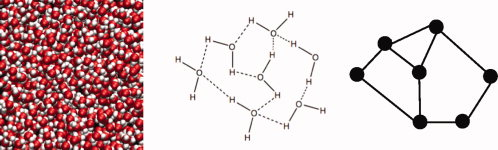
\includegraphics[width=\linewidth]{Decomposition_of_simulation_date_into_a_graph_-chem.jpg}
\caption{Decomposition of simulation data into a graph, taken from \cite{JCC:JCC22917}}
\label{fig:chem}
\end{figure}
We are able to assess changes to the Hydrogen bond network due to the solute through the analysis of the network structure, as a graph is formed where the nodes are water molecules, and links represent potential hydrogen bonds, as shown in Figure \ref{fig:chem}. PageRank of each water molecule is determined by the number of edges connected to it, along with the number of edges connected to the nodes neighbours. As each polyhedron has its own unique PR vector, we are able to access a database in order to confirm the polyhedra structure. The use of PageRank is a novel way to extract chemical information, and can enhance the traditional methods used in chemical spectroscopy.
